\documentclass{ximera}
\title{Curve Sketching}
\begin{abstract}
\end{abstract}
\begin{document}
\maketitle
\section{Introduction}
\begin{dialogue}
\item[Dylan] Using CAS systems to graph is great and all, but on a test where I don't have a calculator it's so hard to sketch a curve!
\item[James] Well maybe we can use derivatives to figure out properties of the graph so it's easier to sketch!
\item[Dylan] Oh! We'd be able to see where the graph was heading up or down, plus we'd be able to see extrema when the derivative at a point is zero!
\end{dialogue}

\section{Guided Problems}

\begin{question}
Consider the function $f(x)=x^3+12x^2+4$.
Take the derivative and find the values where $f'(x)=0$. Create a number line, and mark these points. Between them, mark the sign of the derivative of any point on that interval (Do this by hand). An example is shown below.

\begin{image}
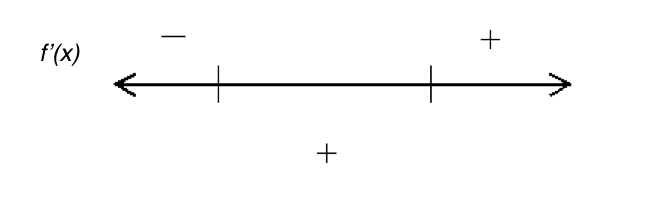
\includegraphics{ExampleNumberline}
\end{image}

On what interval(s) is the derivative positive?

\begin{selectAll}
\choice{$[-8, 0)$}
\choice[correct]{$(-\infty,-8)$}
\choice{$(-\infty, 0]$}
\choice[correct]{$(0,\infty)$}
\end{selectAll}

On what interval(s) is the derivative negative?

\begin{selectAll}
\choice{$[-4, \infty)$}
\choice[correct]{$(-8,0)$}
\choice{$(-\infty, 0]$}
\choice{$(0,\infty)$}
\end{selectAll}

Select everything you can always say about the graph of a function at a point where the derivative is 0:

\begin{selectAll}
\choice[correct]{The graph will be flat at that point.}
\choice{The derivative will change from positive to negative at the point.}
\choice{The derivative will change from negative to positive at the point.}
\choice{The derivative will change sign going from one side of the point to the other.}
\end{selectAll}
\begin{feedback}[correct]
If the derivative at a point is zero, we can only tell that the graph flattens out. It is possible that the sign does not change after crossing the point!
\end{feedback}
\end{question}

\begin{dialogue}
\item[Julia] So we have local maxima or minima when the derivative is 0, but what about the graph of $x^3$?
\end{dialogue}

\begin{image}
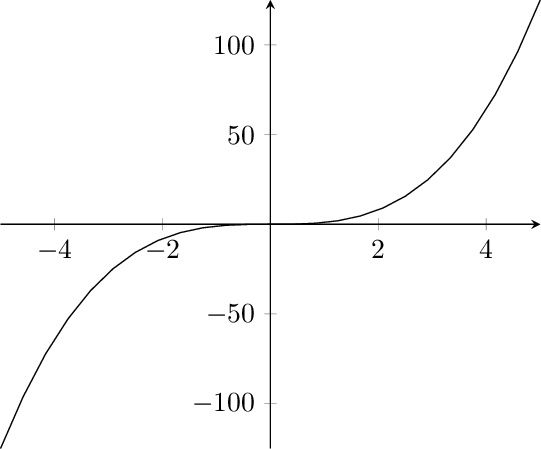
\includegraphics[scale=.3]{00001}
\end{image}

\begin{dialogue}
\item[Dylan] Hmmm...I guess that means there are three different kinds of critical points! Two when the sign changes and one when it stays the same!
\item[Julia] Wait... what's a critical point?
\item[Dylan] A \textbf{critical point} is any point where the derivative is zero or does not exist! Because we know it's important, but we have to check to see what it means with our number line!

\item[James] You guys are still figuring that out? I'm already determining concavity!
\item[Dylan and Julia] Holy cat fur! What's concavity?!
\item[James] A graph is \textbf{concave up} when its derivative is increasing, and \textbf{concave down} when its derivative is decreasing. The easiest way to tell is to look at the curve and think `Would this hold water?' If it would, it's concave up, and if not, it's concave down!
\item[Dylan and Julia] Wow! Thanks James!
\end{dialogue}
\begin{question}

Now determine the second derivative, $f''(x)$, of our original function $f(x) = x^3 + 12x^2+4$. What happens at the points where the second derivative is zero?

\begin{multipleChoice}
\choice{They show the function is at extrema as well.}
\choice{They indicate that concavity will remain the same.}
\choice[correct]{They indicate that concavity is changing.}
\choice{They show that the function is at minimum change.}
\end{multipleChoice}
\vspace{10mm}

Points where concavity changes are known as \textbf{inflection points}.

Draw another number line, this time for the second derivative, marking where the derivative equals zero. Evaluate $f''(x)$ on a point of each of the intervals created through this marking, and mark the sign. What might this mean in general for changing signs on each side of an inflection point?

\begin{selectAll}
\choice{The graph will be flat at that point.}
\choice{The concavity will change from up to down at the point.}
\choice{The concavity will change from down to up at the point.}
\choice[correct]{The concavity will change in that point, but it is impossible to tell how without knowing the value of the

second derivative around that point.}
\end{selectAll}
\vspace{5mm}
Where is the graph concave up?
\begin{multipleChoice}
\choice{$[0,1]$}
\choice[correct]{$(-4, \infty)$}
\choice{$(-\infty, 0)$}
\choice{$[0,260]$}
\choice{$[4,260]$}
\end{multipleChoice}
\vspace{5mm}
What about concave down?

\begin{multipleChoice}
\choice{$[0,1]$}
\choice{$[-4, \infty)$}
\choice[correct]{$(-\infty, -4)$}
\choice{$[0,260]$}
\choice{$[4,260]$}
\end{multipleChoice}
\vspace{5mm}

Inflection points are given as ordered pairs. Evaluate each inflection point you found using $f(x)$ to determine the ordered pairs, then select them below.
\begin{selectAll}
\choice[correct]{$(-4,132)$}
\choice{$(0, 4)$}
\choice{$(-12.028, 0)$}
\choice{$(-8,260)$}
\end{selectAll}
\vspace{5mm}
Based on what you've done until now, sketch the graph yourself. When you're done, click below to see the graph.

\begin{multipleChoice}
\choice[correct]{I'm Done! Show me the graph!}
\end{multipleChoice}
\begin{feedback}
\[
\graph[height=400,xmin=-50,xmax=50,ymin=-300,ymax=500]{x^3+12x^2+4}
\]
\end{feedback}
\end{question}
\begin{dialogue}
\item[Julia] Wait but what about the graph of $f(x)=x^4$? $f''(x)=0$ at the origin but the graph doesn't change concavity see?
\[
\graph[height=400,xmin=-2,xmax=2,ymin=-0.5,ymax=2]{x^4,12x^2}
\]
\item[Dylan] Oh jeez, does that mean that not every instance of $f''(x)=0$ is an inflection point?
\item[James] Not always! That's why you have to make another number line for the second derivative to see if the sign of $f''(x)$ changes on either side of the point where $f''(x)=0$.
\end{dialogue}
\section{On Your Own}
\begin{question}
Now, consider the function $$f(x)=x^{2/3}(6-x)^{1/3}\text{.}$$ Without graphing the function, complete the following:

Select each type of extrema present on the graph.
\begin{selectAll}
\choice[correct]{Local Maximum}
\choice[correct]{Local Minimum}
\choice{Global Maximum}
\choice{Global Minimum}
\end{selectAll}

Indicate the coordinates of any critical points.
\begin{selectAll}
\choice{(-6,0)}
\choice[correct]{(6,0)}
\choice{(3.175, 4)}
\choice[correct]{(4,3.175)}
\choice{(1,3)}
\choice[correct]{(0,0)}
\choice{(5,0)}
\end{selectAll}

Indicate the coordinates of any inflection points.
\begin{selectAll}
\choice{(-6,0)}
\choice[correct]{(6,0)}
\choice{(3.175, 4)}
\choice{(4,3.175)}
\choice{(1,3)}
\choice{(0,0)}
\choice{(5,0)}
\end{selectAll}

Select the intervals on which the function is concave up.
\begin{selectAll}
\choice{$(-\infty), 0)$}
\choice{$(0,6)$}
\choice{$(0,\infty)$}
\choice[correct]{$(6, \infty)$}
\end{selectAll}

Select the intervals on which the function is concave down.

\begin{selectAll}
\choice[correct]{$(-\infty), 0)$}
\choice[correct]{$(0,6)$}
\choice{$(0,\infty)$}
\choice{$(6, \infty)$}
\end{selectAll}


Now, create a sketch of your function on paper. When you're done, click below to see how your graph should look!

\begin{multipleChoice}
\choice[correct]{I'm done waiting! Show me the graph!}
\choice{I'm not ready yet, but I'm going to click regardless!}
\end{multipleChoice}
\begin{feedback}[correct]
\[
\graph[height=400,ymin=-5,ymax=5,xmin=-5,xmax=10]{x^{2/3}(6-x)^1/3}
\]
\end{feedback}
\end{question}

\begin{question}
Now, consider the function $$f(x)=x^3-3x+5\text{.}$$ Without graphing the function, complete the following:

Select each type of extrema present on the graph.
\begin{selectAll}
\choice[correct]{Local Maximum}
\choice[correct]{Local Minimum}
\choice{Global Maximum}
\choice{Global Minimum}
\end{selectAll}

Indicate the coordinates of any critical points.
\begin{selectAll}
\choice{(-2,0)}
\choice[correct]{(-1,7)}
\choice{(-3,7)}
\choice{(7,-2)}
\choice[correct]{(1,3)}
\choice{(0,5)}
\choice{(5,0)}
\end{selectAll}

Indicate the coordinates of any inflection points.
\begin{selectAll}
\choice{$(-2,0)$}
\choice{$(-1,7)$}
\choice{$(-3,7)$}
\choice{$(7,-2)$}
\choice{$(1,3)$}
\choice[correct]{$(0,5)$}
\choice{$(5,0)$}
\end{selectAll}

Select the intervals on which the function is concave up.
\begin{selectAll}
\choice{$[-5,10]$}
\choice{$[1,2]$}
\choice[correct]{$(0,\infty)$}
\choice{$(-\infty, 0)$}
\end{selectAll}

Select the intervals on which the function is concave down.

\begin{selectAll}
\choice{$[0,10]$}
\choice{$[1,2]$}
\choice{$[0,\infty)$}
\choice[correct]{$(-\infty,0]$}
\end{selectAll}

Now, create a sketch of your function on paper. When you're done, click below to see how your graph should look!

\begin{multipleChoice}
\choice[correct]{I'm done waiting! Show me the graph!}
\choice{I'm not ready yet, but I'm going to click regardless!}
\end{multipleChoice}
\begin{feedback}[correct]
\[
\graph[height=400,ymin=-5,ymax=15,xmin=-10,xmax=10]{x^3-3x+5}
\]
\end{feedback}
\end{question}


\section{Matching Graphs}
\begin{dialogue}
\item[Dylan]So if I wanted to match a graph with the graphs of its first and second derivative I can do that now!
\item[Julia] Wait, really?? How?
\item[James] Well the $y$ value of $f'(x)$ corresponds to the slope of $f(x)$, and the $y$ value of $f''(x)$ corresponds to the slope of $f'(x)$ and is related to the concavity of $f(x)$.
\item[Julia] So we can match the graphs based on how all that information relates!
\item[Dylan] Exactly, let's try it!
\end{dialogue}
\begin{question}
For the following problems, select the correct match of $f(x),f'(x), and f''(x)$

\begin{multipleChoice}
\choice{\begin{image}
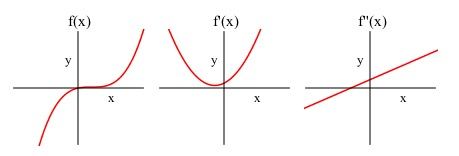
\includegraphics{nope3.jpg}
\end{image}}
\choice[correct]{\begin{image}
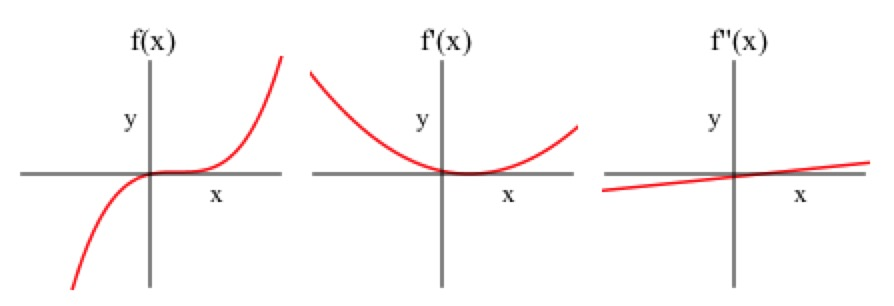
\includegraphics{match1.jpg}
\end{image}}
\choice{\begin{image}
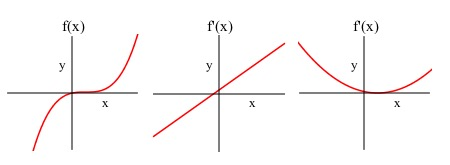
\includegraphics{nope1.jpg}
\end{image}}
\choice{\begin{image}
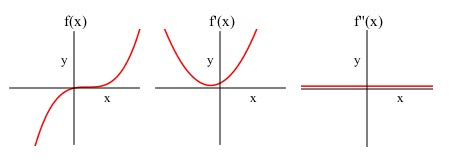
\includegraphics{nope2.jpg}
\end{image}}
\end{multipleChoice}

\begin{multipleChoice}
\choice{\begin{image}
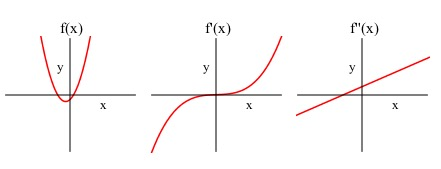
\includegraphics{2a.jpg}
\end{image}}
\choice{\begin{image}
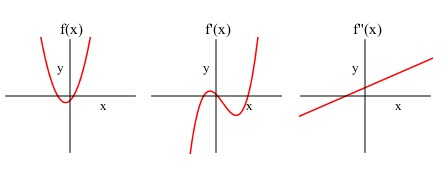
\includegraphics{2c.jpg}
\end{image}}
\choice{\begin{image}
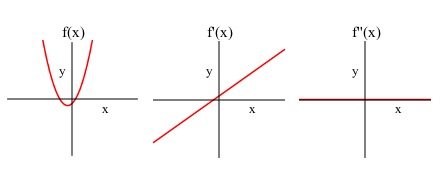
\includegraphics{2b.jpg}
\end{image}}
\choice[correct]{\begin{image}
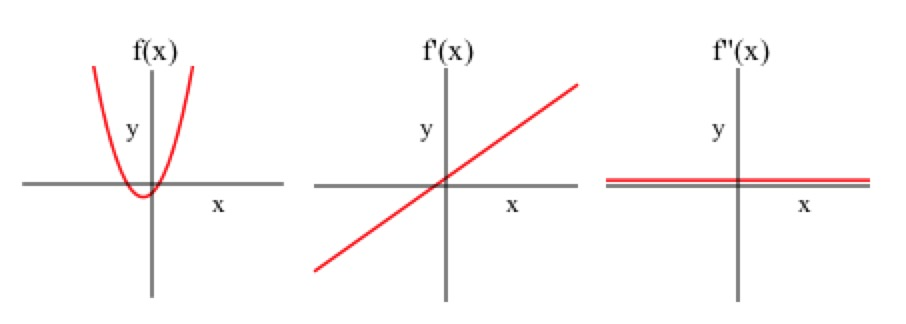
\includegraphics{match2.jpg}
\end{image}}
\end{multipleChoice}

\begin{multipleChoice}
\choice{\begin{image}
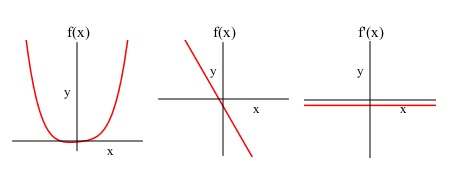
\includegraphics{3c.jpg}
\end{image}}
\choice{\begin{image}
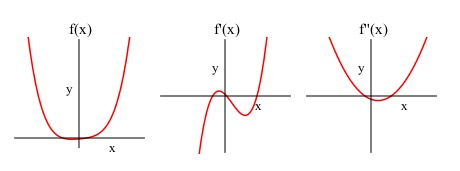
\includegraphics{3a.jpg}
\end{image}}
\choice[correct]{\begin{image}
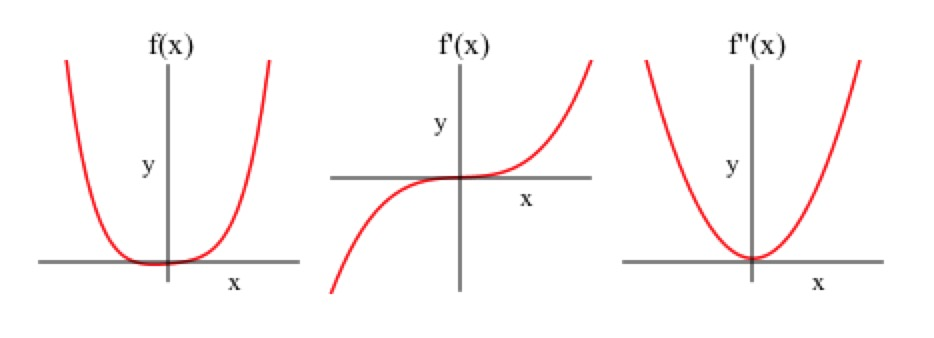
\includegraphics{match3.jpg}
\end{image}}
\choice{\begin{image}
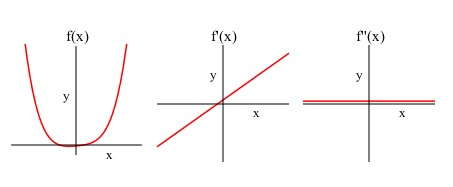
\includegraphics{3b.jpg}
\end{image}}
\end{multipleChoice}

\begin{multipleChoice}
\choice[correct]{\begin{image}
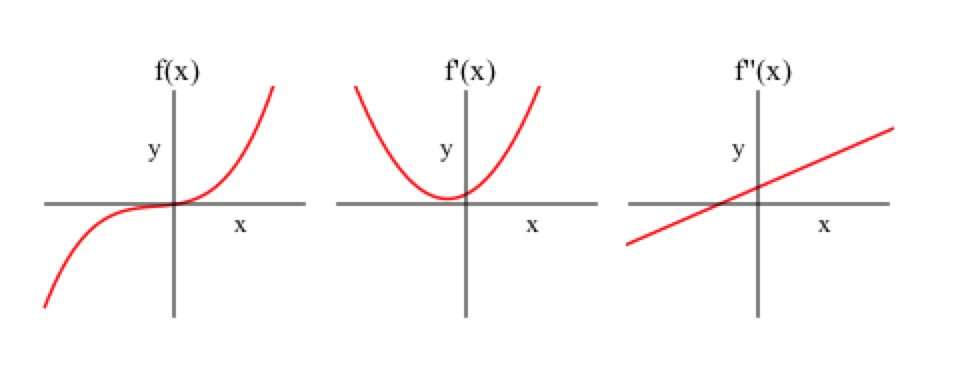
\includegraphics{match4.jpg}
\end{image}}
\choice{\begin{image}
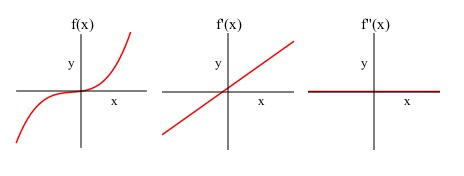
\includegraphics{4c.jpg}
\end{image}}
\choice{\begin{image}
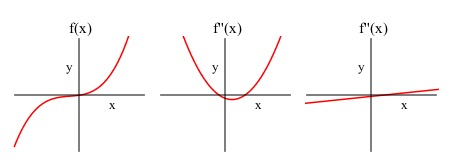
\includegraphics{4a.jpg}
\end{image}}
\choice{\begin{image}
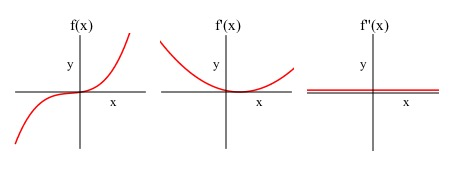
\includegraphics{4b.jpg}
\end{image}}
\end{multipleChoice}

\end{question}


\section{In Summary}
In this lab, you've covered quite a bit. To help organize everything, we've put the important theorems below.

We've also included the second derivative test below, which is another method to determine if a critical point is a maximum, minimum, or saddle point. To do this, you simply evaluate the second derivative at the critical point, and determine what that point is based on the value, as shown in the table.

\begin{theorem}[First Derivative Test]
Suppose that $c$ is a critical number($f'(c)=0$) on a continuous function $f$.
\begin{enumerate}
\item If $f'$ changes from positive to negative at $c$, then $f$ has a local maximum at $c$.
\item If $f'$ changes from negative to positive at $c$, then $f$ has a local minimum at $c$.
\item If $f'$ does not change sign at $c$, then $f$ has a saddle point at $c$.
\end{enumerate}
\begin{remark}
When $f'(c)$ does not exist:
\begin{enumerate}
\item{If $c$ is in the domain of $f$, follow the same steps as when $f'(c)=0\text{.}$}
\item{If $c$ is not in the domain, then $c$ is not a critical number.}
\end{enumerate}
\end{remark}
\end{theorem}

\begin{theorem}[Concavity Test]
If $f''(x)$ exists for all $x\in(a,b)$ 
\begin{enumerate}
\item{If $f''(x)>0$ for all $x\in(a,b)$, then $f$ is concave up on $(a,b)$}
\item{If $f''(x)<0$ for all $x\in(a,b)$, then $f$ is concave down on $(a,b)$}
\end{enumerate}
\end{theorem}

\begin{theorem}[Test for Inflection Points]
If $f''(c)=0$ or $f''(c)$ does not exist and $f''(x)$ changes sign at $x=c$, then $f$ has a point of inflection at $x=c$
\end{theorem}

\begin{theorem}[Second Derivative Test]
Let $c$ be a critical point of $f(x)$. If $f''(c)$ exists, then
\begin{enumerate}
\item{If $f''(c)>0$, then $f(c)$ is a local minimum.}
\item{If $f''(c)<0$, then $f(c)$ is a local maximum.}
\item{If $f''(c)=0$, then the test is inconclusive: $f(c)$ could be a local max, min, or neither.}
\end{enumerate}
\end{theorem}
\end{document}
%\pagebreak